% !TeX spellcheck = en_US
\documentclass[a4paper,12pt]{article}
\usepackage[utf8x]{inputenc}
\usepackage{wrapfig}
\usepackage{graphicx}
\usepackage{float}
\usepackage{listings}
\usepackage{amsmath}
\usepackage{caption}
\usepackage{subcaption}
\usepackage[usenames,dvipsnames,svgnames,table]{xcolor}

% Title Page
\title{AST2210 Report 3}
\author{Andreas Ellewsen}

\begin{document}
\maketitle
\section{Introduction}
In this lab exercise we will go through the most common types of aberrations. This includes chromatic aberration and the Seidel aberrations. There are five Seidel aberrations; spherical aberration, coma, astigmatism, curvature of field, and distortion. The focus of this lab is spherical aberration, coma and astigmatism.
\section{Setup}
A laser is connected to a tube. The light passes through this tube, and then through a thin singlet lens. After the lens, an objective is placed. At the end of this the camera is placed. The lens and objective is moved relative to each other so that the focus point hits the CCD in the camera.
\section{Chromatic aberration}
Chromatic aberration is the phenomenon that light with different wavelengths have different focal points along the optical axis.
The distance between the different focal points were found to be $0.3 \pm 0.1 cm$. The three different maximum can be seen in figure \ref{fig:Chromatic abberations}. A quick look at each of them reveals a clear Airy pattern. This pattern occurs when light passes through a small circular aperture. The formula for the first minimum is $sin(\theta) = \frac{1.22\lambda}{d}$, where $d$ is the diameter of the aperture, and $\lambda$ is the wavelength of the light. 
\begin{figure}[H]
        \centering
        \begin{subfigure}{0.3\textwidth}
                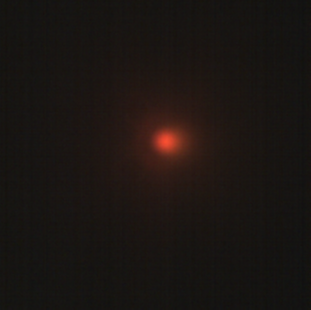
\includegraphics[width=\textwidth]{redfocus}
                \caption{Red airy disk}
                \label{fig:redfocus}
        \end{subfigure}
        \begin{subfigure}{0.3\textwidth}
                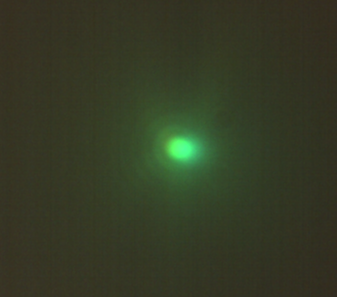
\includegraphics[width=\textwidth]{greenfocus}
                \caption{Green airy disk}
                \label{fig:greenfocus}
        \end{subfigure}%
        ~ %add desired spacing between images, e. g. ~, \quad, \qquad, \hfill etc.
          %(or a blank line to force the subfigure onto a new line)
        \begin{subfigure}{0.3\textwidth}
                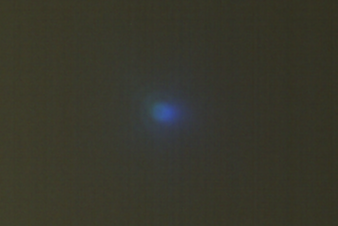
\includegraphics[width=\textwidth]{bluefocus}
                \caption{Blue airy disk}
                \label{fig:bluefocus}
        \end{subfigure}
        \caption{The three focal points}\label{fig:Chromatic abberations}
\end{figure}

\section{Spherical aberration}
This aberration is caused by the effect that annuli of a lens that are of different radii have different focal lengths. We use the same set-up as the previous exercise with the same thin singlet lens and color camera, but now with the laser connected to the collimator tube (with dampening filter). The reason for using a singlet lens is that it has more spherical aberration than doublet lenses. Doublet lenses are designed to reduce spherical aberration almost to zero. The result can be seen in figure \ref{fig:Spherical aberrations}. And they are as expected. Figure \ref{fig:sainside} shows it inside focus. Here we get these sharp edges. Figure \ref{fig:sain} shows the Airy disk in focus. Figure \ref{fig:saout} shows the disk outside focus, where we get a blurring effect.
\begin{figure}[H]
        \centering
        \begin{subfigure}{0.3\textwidth}
                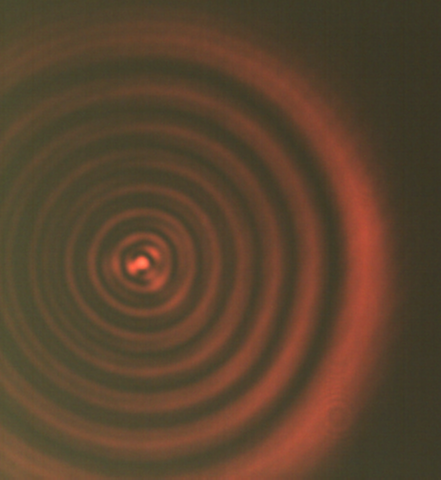
\includegraphics[width=\textwidth]{airyinsidefocus}
                \caption{Inside focus}
                \label{fig:sainside}
        \end{subfigure}
        \begin{subfigure}{0.3\textwidth}
                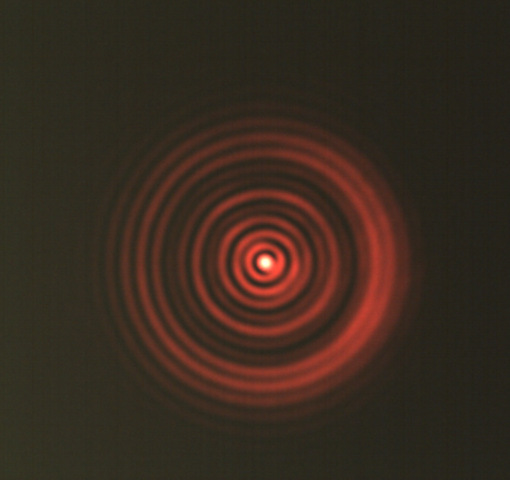
\includegraphics[width=\textwidth]{airyinfocus}
                \caption{In focus}
                \label{fig:sain}
        \end{subfigure}%
        ~ %add desired spacing between images, e. g. ~, \quad, \qquad, \hfill etc.
          %(or a blank line to force the subfigure onto a new line)
        \begin{subfigure}{0.3\textwidth}
                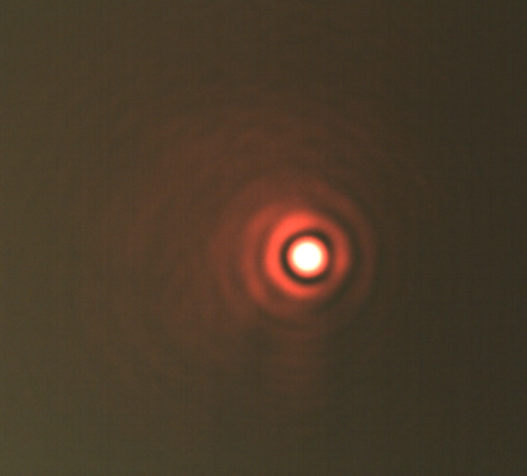
\includegraphics[width=\textwidth]{airyoutfocus}
                \caption{Outside focus}
                \label{fig:saout}
        \end{subfigure}
        \caption{Spherical aberrations}\label{fig:Spherical aberrations}
\end{figure}

\section{Coma}
Coma is an aberration which causes rays from an off-axis point of light in the object plane to create a trailing "comet-like" blur directed away from the optical axis. According to the lab text, lenses with coma are hard to come by nowadays, and so we have a specifically designed lens for the purpose of this exercise. The pictures taken in the lab can be seen in figures \ref{fig:Coma1} and \ref{fig:Coma2}. To make these pictures, we tilted the lens until the "comet trail" showed up.

\begin{figure}[H]
        \centering
        \begin{subfigure}{0.3\textwidth}
                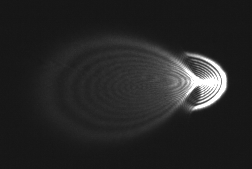
\includegraphics[width=\textwidth]{comastor}
                \caption{Coma big}
                \label{fig:comastor}
        \end{subfigure}
        \begin{subfigure}{0.3\textwidth}
                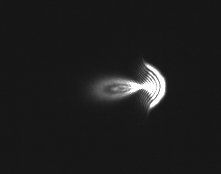
\includegraphics[width=\textwidth]{comaliten}
                \caption{Coma small}
                \label{fig:comaliten}
        \end{subfigure}%
        ~ %add desired spacing between images, e. g. ~, \quad, \qquad, \hfill etc.
          %(or a blank line to force the subfigure onto a new line)
        \begin{subfigure}{0.3\textwidth}
                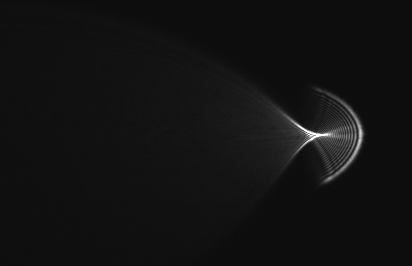
\includegraphics[width=\textwidth]{comahoyre2}
                \caption{Coma right}
                \label{fig:comahoyre}
        \end{subfigure}
        \caption{Examples of coma}\label{fig:Coma1}
\end{figure}

\begin{figure}[H]
        \centering
        \begin{subfigure}{0.3\textwidth}
                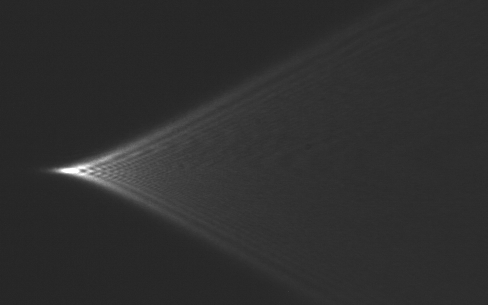
\includegraphics[width=\textwidth]{comavenstre2}
                \caption{Coma left}
                \label{fig:comavenstre}
        \end{subfigure}
        \begin{subfigure}{0.3\textwidth}
                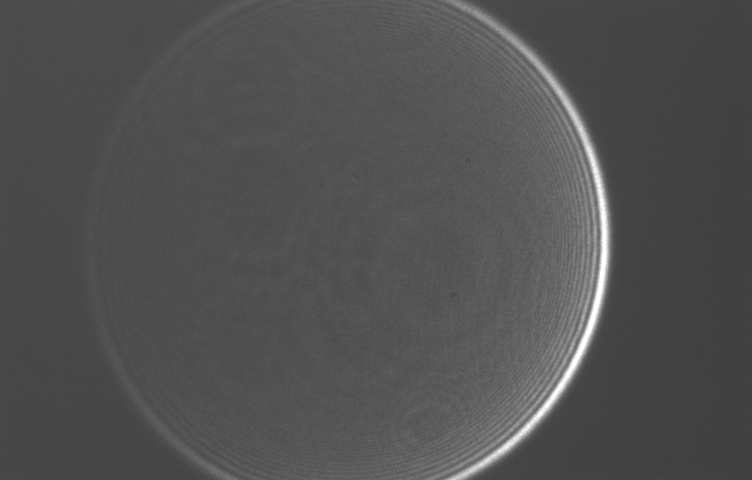
\includegraphics[width=\textwidth]{comamidt}
                \caption{Coma middle}
                \label{fig:comamidt}
        \end{subfigure}%
        ~ %add desired spacing between images, e. g. ~, \quad, \qquad, \hfill etc.
          %(or a blank line to force the subfigure onto a new line)
        \begin{subfigure}{0.3\textwidth}
                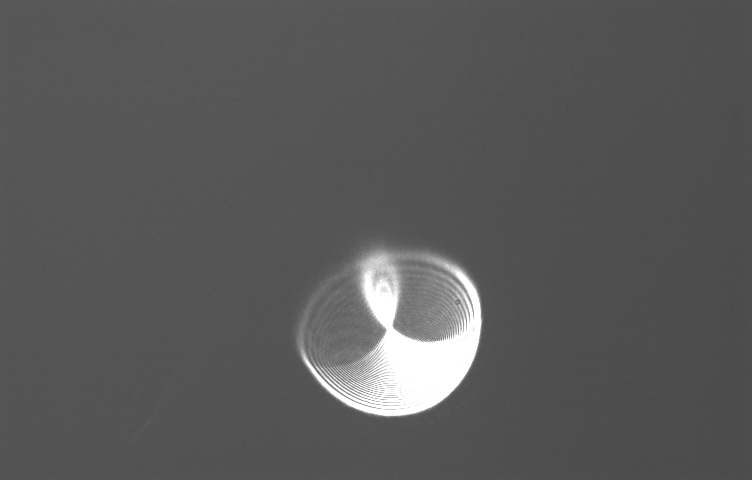
\includegraphics[width=\textwidth]{comaned}
                \caption{Coma down}
                \label{fig:comaned}
        \end{subfigure}
        \caption{More examples of coma}\label{fig:Coma2}
\end{figure}
When using an aperture to block light one can see that the size of the rings decrease while the number of rings stays the same. Which means the distance between the rings is decreasing.
 
\section{Astigmatism}
Astigmatism is an aberration for which in the case of an off-axis object, rays in different planes have different foci. The planes to consider are the tangential plane: the plane containing the object and the optical axis, and the sagittal plane: the plane perpendicular to the tangential plane. In a system with astigmatism, a point source becomes a cross. To illustrate astigmatism, we use a thick doublet lens in the set-up with the laser, collimator tube with dampening filter and mono-chromatic camera. The lens is then titled in different directions, to get different examples of the effect. The pictures can be seen in figure \ref{fig:Astigmatism}

\begin{figure}[H]
        \centering
        \begin{subfigure}{0.3\textwidth}
                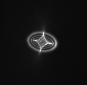
\includegraphics[width=\textwidth]{astig_1}
                \caption{Astigmatism}
                \label{fig:astig1}
        \end{subfigure}
        \begin{subfigure}{0.3\textwidth}
                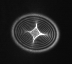
\includegraphics[width=\textwidth]{astig_2}
                \caption{Astigmatism}
                \label{fig:astig2}
        \end{subfigure}%
        ~ %add desired spacing between images, e. g. ~, \quad, \qquad, \hfill etc.
          %(or a blank line to force the subfigure onto a new line)
        \begin{subfigure}{0.3\textwidth}
                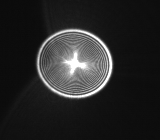
\includegraphics[width=\textwidth]{astig_3}
                \caption{Astigmatism}
                \label{fig:astig3}
        \end{subfigure}
        \caption{Examples of astigmatism}\label{fig:Astigmatism}
\end{figure}

\section{Distortion}
This section was supposed to demonstrate barrel distortion. However, there was not enough time to do this, and we couldn't find the lens needed for the setup. Barrel distortion magnifies the picture, with the magnification decreasing with the distance from the optical axis.

\section{Summary}
In this lab we've gone through some of the most common optical aberrations. We've seen that different wavelengths of light have different focal points along the optical axis. We've seen the blurring and sharpening\footnote{Sharpening here does not make the picture better. I'm just unsure of what word to use to describe the effect seen in the picture. If you look at the pictures in the part about spherical aberration, you can hopefully see what I mean.} of spherical aberrations. Then we studied the "comet-like" blur in lenses with coma. Here we also studied the effects caused by putting an aperture in the optical path and decreasing the size of it. And finally we studied astigmatism and got some nice pictures of the cross caused by it.
\end{document}